\documentclass[a4paper, 10pt]{article}
\usepackage[utf8]{inputenc}
\usepackage[spanish]{babel}
\usepackage{graphicx}
\usepackage{geometry}
\usepackage{listings}
\usepackage{amsmath}
\usepackage{amsfonts}
\usepackage{amssymb}
\usepackage{caratula}

\newcommand{\Z}{\mathbb{Z}}
\def\code#1{\texttt{#1}}
\newcommand\tab[1][0.5cm]{\hspace*{#1}}

\geometry{a4paper, margin=0.7in}

\begin{document}
    %Caratula
    \pagenumbering{gobble}
    \newpage

    \begin{center}
        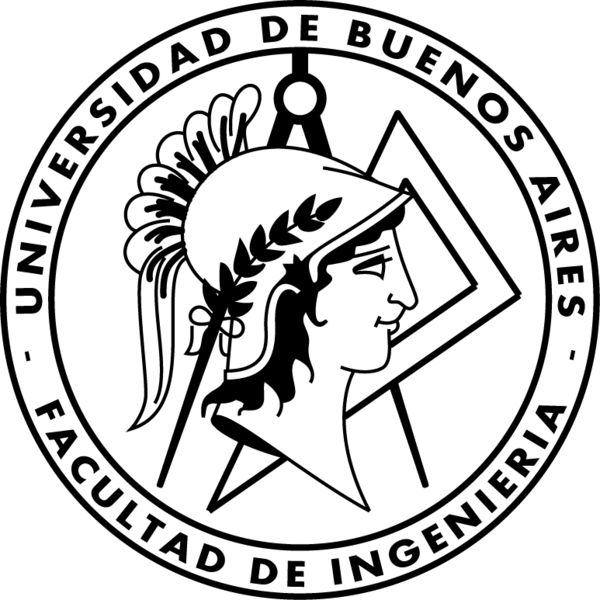
\includegraphics[width=7.5cm, height=7.5cm]{images/logo}
    \end{center}

    \materia{Organización de Datos}
    \submateria{Segundo Cuatrimestre 2017}
    \titulo{Trabajo Práctico 1}

    \integrante{Rodrigo De Rosa}{97799}{rodrigoderosa@outlook.com}
    \integrante{Marcos Schapira}{97934}{schapiramarcos@gmail.com}
    \integrante{Facundo Guerrero}{97981}{facundoiguerrero@gmail.com}
    \maketitle
    %Fin caratula
    %Table of contents
    \newpage
    \pagenumbering{roman}
    \tableofcontents
    %Fin table of contents
    %Informe
    \newpage
	\pagenumbering{arabic}
	\part{Análisis del precio por $m^2$}
		\section{Adaptación del DataFrame}
			Para el análisis particular de cada característica de la información que se posee, se adaptó el DataFrame
			original para poder analizar dicha información mas fácil y comodamente.
			\subsection{Filtrado de columnas}
				Para el análisis de esta cierta característica de las propiedades, consideramos \emph{importantes}
				sólo a algunas celdas. Estas son:
				\begin{itemize}
					\item \code{place name} $\leftarrow$ \code{location}
					\item \code{price aprox usd} $\leftarrow$ \code{price}
					\item \code{surface total in m2} $\leftarrow$ \code{totalSurface}
					\item \code{surface covered in m2} $\leftarrow$ \code{coveredSurface}
					\item \code{price usd per m2} $\leftarrow$ \code{pricem2}		
				\end{itemize}
			\subsection{Completando el DataFrame}
				Lo primero que se hizo para realizar este analisis fue completar las columnas faltantes
				de la mayor cantidad de entradas posibles. Esto es, \code{location, price, totalSurface,
				pricem2}. De esta forma, nos permitimos analizar una mayor cantidad de propiedades
				para realizar un analisis un poco mas correcto. \\
				\tab Para completar el campo de precio por $m^2$ se necesita que la entrada sobre la que
				se trabaja cumpla la siguiente condición lógica: $price_{}m^2 \vee (price \wedge surface)$. Es
				decir, necesita tener o el precio por metro cuadrado o tanto el precio total como la superficie
				total. \\
				\tab Si el campo \code{pricem2} tiene valor, entonces ese será el utilizado. En caso contrario,
				si tanto el campo \code{price} como el campo \code{totalSurface} tienen valor, definimos como
				nuestro nuevo \code{pricem2} a la división $\frac{price}{surface}$. \\
				\tab Para esto, necesitamos unificar \code{coveredSurface} y \code{totalSurface}, para maximizar
				nuevamente la cantidad de entradas disponibles. Esto se hace, simplemente, poniendo como
				\code{totalSurface} el valor de \code{coveredSurface} en aquellas entradas donde la primera
				no tenga valor (consideramos que $total - covered = uncovered$). \\
				\tab Una vez completados todos los \code{pricem2} posibles, eliminamos todas aquellas entradas
				que tengan \code{NaN} como valor (en cualquiera de las celdas que definimos como \emph{importantes}),
				pues ya no podemos obtener el valor de esa celda de ningun otro lugar.
		\section{Estudio estadístico de los datos}
			\subsection{Analisis de la distribución de precios}
				Una vez completado el DataFrame lo mas posible, se realizó un análisis de la distribución de precios.
				Con esto nos referimos a analizar la variación del precio por metro cuadrado entre todas las
				propiedades. Es decir, \emph{limpiar los datos que no tienen sentido}. \\
				\tab Para esto le pedimos el \code{.describe()} a nuesto DataFrame con los percentiles $0.01$ y
				$0.99$. Esto nos permite analizar que tan desviados estan los valores máximos y mínimos. \\
				\tab Con los percentiles recién mencionados hacemos un recorte de los datos para lograr una distribución
				que se asemeje a una Normal lo mas posible. El primer recorte es tanto inferior ($ > 150USD$) como superior
				($<18000USD$). Como en este nuevo DataFrame la diferencia entre el percentil $0.99$ y el máximo es de más
				del doble, se vuelve a recortar superiormente ($<8000USD$). \\
				\tab Luego de esto, la distribución de precios es un poco mejor que antes (las diferencias entre los
				percentiles $0.25, 0.5, 0.75$ son similares). \\
				\tab A continuación se muestra un gráfico de distribución de precios por metro cuadrado que se obtiene
				del DataFrame original sin realizar el filtrado recién mencionado. Nos hubiese gustado poder mostrar tanto
				el KDE como el histograma pero al haber tanta diferencia entre el maximo y los valores principales de la
				distribución, el histograma era solo una linea. El objetivo de este gráfico es hacer incapié en lo mencionado
				en el previo párrafo: es necesario filtrar los datos para tener un conjunto de datos con sentido.
				\begin{center}
       				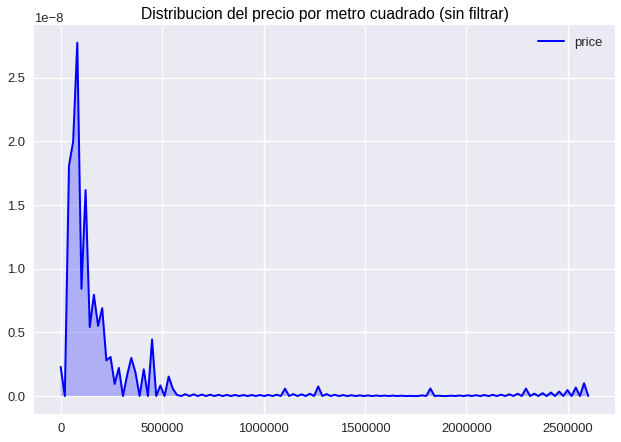
\includegraphics[width=6in, height=4in]{images/m2UnfilteredKDE}
		   		\end{center}
				\tab En el siguiente gráfico de distribución de precios por metro cuadrado se puede ver que la mayor parte
				de las propiedades están concentradas en el rango de precios $[150;4000]USD$ y luego hay un drástico decaimiento
				de cantidad de propiedades para el resto de los precios. Si bien se podría considerar que un recorte sería
				correcto, a partir de fuentes externas se sabe que ciertos barrios (\emph{i.e.} Puerto Madero) tienen,
				aproximadamente, un valor medio de $6000USD$ por metro cuadrado.
				\begin{center}
       				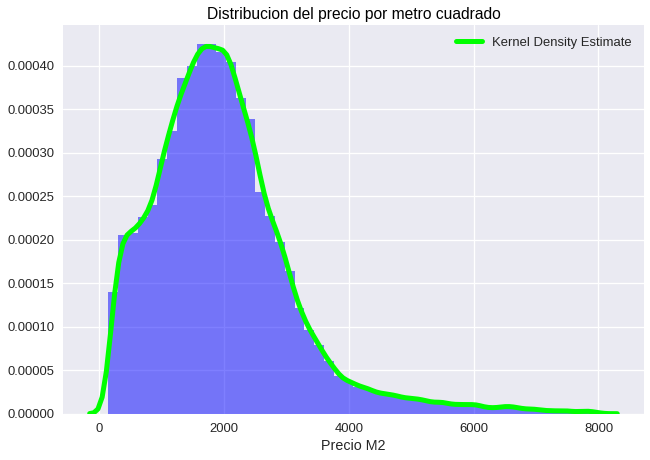
\includegraphics[width=6in, height=4in]{images/m2Histogram}
		   		\end{center}
			\subsection{Agrupando por barrios}
				Ahora que nuestros datos están tan completos y retocados como querríamos, procedemos a agrupar todas las propiedades
				de acuerdo al barrio al que pertencen. Una vez que los tenemos agrupados, debemos establecer un \emph{minimo de
				propiedades} por barrio. Pues un barrio que tiene una o dos propiedades podría alterar el estudio de la
				informacion. \\
				\tab Nuevamente, para esta tarea utilizizamos \code{.describe()} y resolvemos que utilizaremos como cota inferior
				$50$ propiedades (dos mas que el equivalente a una publicación por mes en los últimos cuatro años). \\
				\tab Aquí, al igual que hicimos antes, mostraremos la distribución antes y después del filtro aplicado. Si bien
				en escencia no son tan diferentes, podemos observar que desaparecen algunos barrios de la zona de precios altos.
				\begin{center}
       				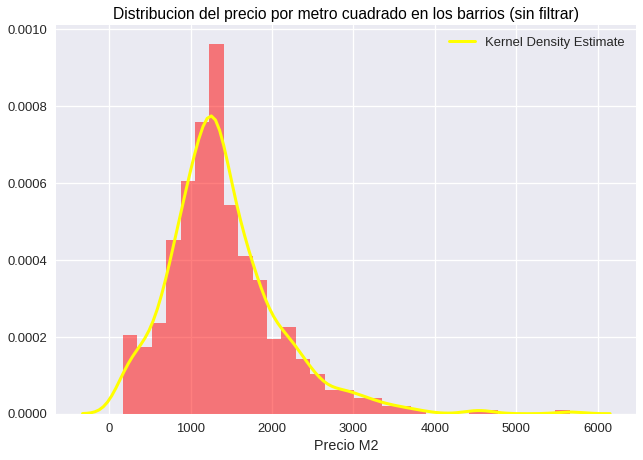
\includegraphics[width=6in, height=4in]{images/m2HoodUnfilteredKDE}
		   		\end{center}
				\tab Una vez que eliminamos los barrios problemáticos, si analizamos la distribución de precio por barrio
				podemos ver que la mayor parte está concentrada en el intervalo $[500;3500]USD$, mientras que muy pocos
				(solo tres) superan ese valor.
				\begin{center}
   	    				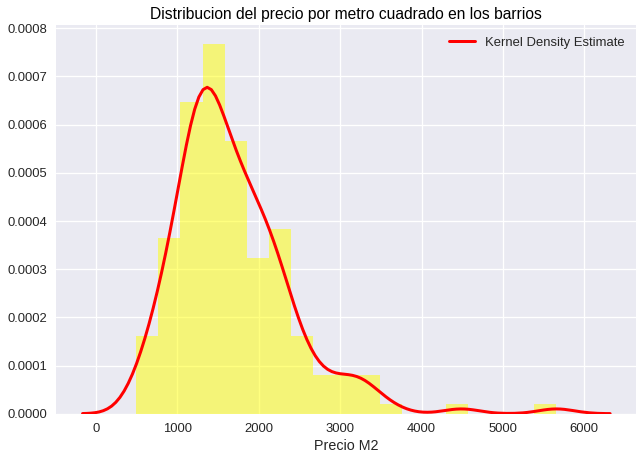
\includegraphics[width=6in, height=4in]{images/m2HoodHistogram}
			    \end{center}	
			    \tab Podemos ver, además, que la distribución es bastante similar a la anterior (sin agrupar por barrios) aunque,
			    obviamente, con valores menores (pues son promedios).
		\section{Analizando grupos característicos}
			En esta sección analizaremos ciertos grupos característicos a partir de la información con la que estamos trabajando.
			\subsection{Los diez barrios con mayor precio por $m^2$}
				Dado que ya estamos felices con la forma en que tenemos dispuestos los datos, comenzaremos por hacer un
				\emph{Top 10} de los barrios más caros de CABA y GBA. \\
				\tab Para esto, como ya tenemos los datos agrupados, simplemente ordenamos el DataFrame y nos quedamos con
				los primeros diez.
				\tab Durante el análisis de esta información, notamos que varios de los barrios que aparecían en este \emph{Top 10}
				eran subdivisiones del barrio de Palermo. Por esta razón, decidimos incluir dos casos: uno en que consideramos
				que todos los 'Palermos' son uno solo, y otro en que cada uno es considerado un barrio diferente.
				\subsubsection{Unificación de Palermo}
					En este caso, consideramos que todas las subdivisiones de Palermo pertenecen a un sólo barrio.\\
					\tab El resultado obtenido es el siguiente:
					\begin{center}
						\begin{tabular}{ |c|c|c| }
							\hline
							\multicolumn{3}{|c|}{Top 10 [Palermo unificado]}\\
							\hline
							Puesto & Barrio & Precio $m^2$ [U$\$$D] \\
							\hline
							1 & Puerto Madero & 5657 \\
							2 & Las Cañitas & 3612 \\
							3 & Palermo & 3518 \\
							4 & Recoleta & 3316 \\
							5 & Belgrano & 3124 \\
							6 & Nuñez & 3056 \\
							7 & Barrio Norte & 2949 \\
							8 & Vicente López & 2925 \\
							9 & Retiro & 2783 \\
							10 & Olivos & 2737 \\
							\hline
						\end{tabular}
					\end{center}
					\tab En la tabla se observa que Puerto Madero tiene un valor mucho mas alto que el resto, de hecho, es
					mayor al doble del precio del décimo. De todos modos, entre el segundo y el último la variación es más
					suave. Para aportar a este análisis, se realiza un gráfico de barras:
					\begin{center}
   	    					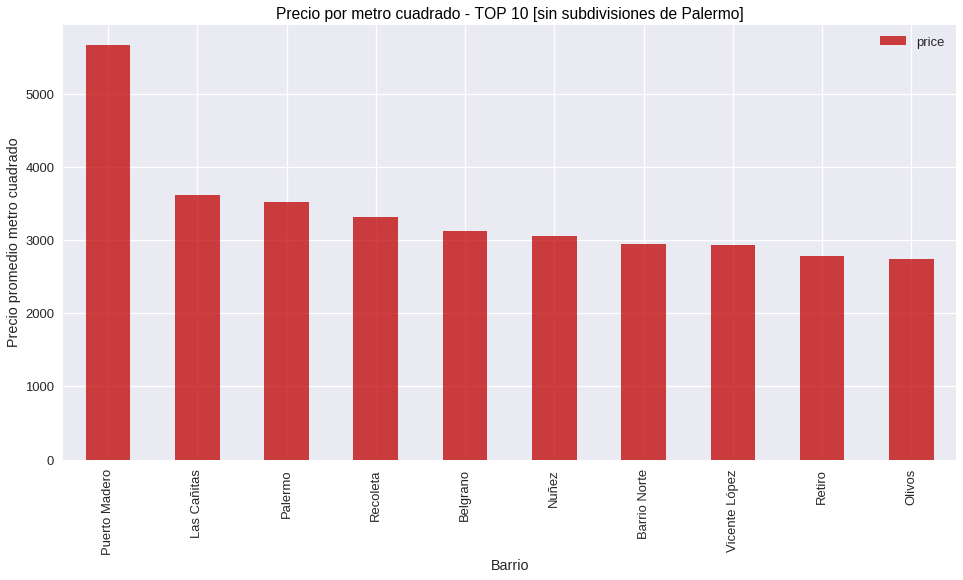
\includegraphics[width=7in, height=3.5in]{images/m2UnifiedTop10}
			  		\end{center}	
			  	\subsubsection{División de Palermo}
			  		Aquí consideraremos que el barrio al que se nombra Palermo corresponde a todas las secciones de dicho
			  		barrio que no son las que ya aparecen en otro grupo. \\
			  		\tab En este caso, el resultado obtenido es:
			  		\begin{center}
						\begin{tabular}{ |c|c|c| }
							\hline
							\multicolumn{3}{|c|}{Top 10 [Palermo dividido]}\\
							\hline
							Puesto & Barrio & Precio $m^2$ [U$\$$D] \\
							\hline
							1 & Puerto Madero & 5657 \\
							2 & Palermo Chico & 4489 \\
							3 & Las Cañitas & 3612  \\
							4 & Palermo Viejo & 3419 \\
							5 & Recoleta & 3316 \\
							6 & Palermo & 3260 \\
							7 & Palermo Hollywood & 3224 \\
							8 & Palermo Soho & 3198 \\
							9 & Belgrano & 3124 \\
							10 & Nuñez & 3056 \\
							\hline
						\end{tabular}
					\end{center}
					\tab En la tabla podemos ver que, si bien es correcto y es un \emph{Top 10}, esta plagado de subdivisiones
					de Palermo y no nos permite tener un plano más general. \\
					\tab Aquí el gráfico de barras es muy similar aunque aparece Palermo Chico, que se acerca un poco mas
					al valor de Puerto Madero. De todos modos, la diferencia entre el primero y el segundo es muy grande
					como también lo es entre el segundo y el tercero, dejando la relación entre los valores igual de 'no suave'.
					\begin{center}
   	    					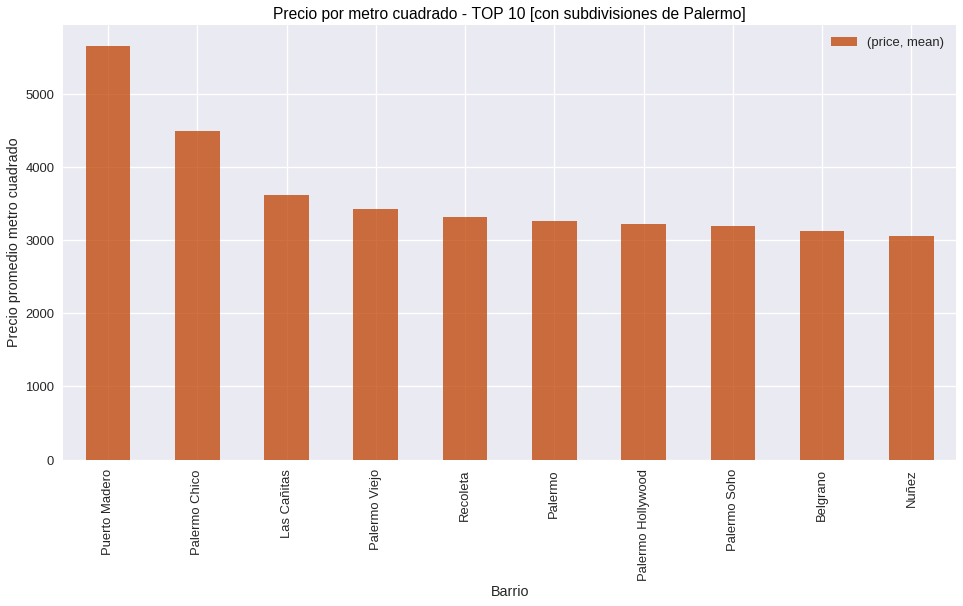
\includegraphics[width=7in, height=3.5in]{images/m2NotUnifiedTop10}
			  		\end{center}
			  		\tab De aquí en más, utilizaremos a Palermo como un barrio unificado.
			  	\subsubsection{Comentario sobre el Top 10}
				  	Este \emph{Top 10} arroja los resultados que se hubieran esperado, pues los únicos dos valores que no pertenecen
			  	a CABA corresponden a los primeros dos barrios de GBA en los que se piensa al pensar en los barrios mas caros
			  	de Buenos Aires. \\
			  		\tab Por otro lado, si nos sorprende el hecho de que el $m^2$ en Barrio Norte sea más barato que Núñez o en
			  		Belgrano.
			\subsection{Los diez barrios con menor precio por $m^2$}
				Para esta parte, al igual que antes, ordenamos los datos para analizar cuales son los diez barrios que se encuentran
				en el \emph{Bottom 10}. \\
				\tab Al realizar este análisis, lo obtenido es:
				\begin{center}
					\begin{tabular}{ |c|c|c| }
						\hline
						\multicolumn{3}{|c|}{Bottom 10}\\
						\hline
						Puesto & Barrio & Precio $m^2$ [U$\$$D] \\
						\hline
						1 & Ingeniero Pablo Nogués & 494 \\
						2 & Maschwitz & 548 \\
						3 & Villa Udaondo & 558 \\
						4 & Parque Leloir & 579 \\
						5 & Presidente Perón & 643 \\
						6 & Benavidez & 705 \\
						7 & José C Paz & 711 \\
						8 & Villa Libertad & 743 \\
						9 & Longchamps & 800 \\
						10 & Burzaco & 804 \\
						\hline
					\end{tabular}
				\end{center}
				\tab Si graficamos estos valores al igual que antes podremos ver un ascenso (o descenso) más suave que el del
				\emph{Top 10}. Si bien el primero es casi la mitad de el último, la variación entre puestos es menor. \\
				\begin{center}
   	    				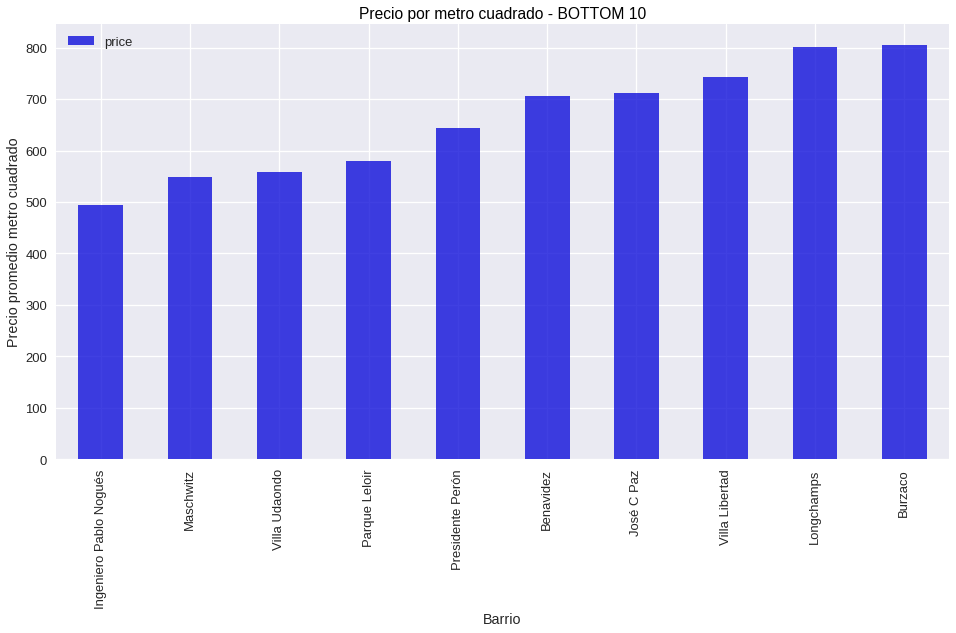
\includegraphics[width=7in, height=3.5in]{images/m2Bottom10}
			  	\end{center}
				\tab Aquí, remitiéndonos a la sección 3.1.3, vemos que los barrios del \emph{Bottom 10} son todos barrios
				alejados de la ciudad, de los cuales es esperable un bajo valor del $m^2$.
			\subsection{Barrios intermedios}
				En esta parte nos dedicaremos a analizar la variación del precio por $m^2$ entre los barrios 'del medio'. Con
				esto nos referimos a aquellos barrios que no están en los extremos sino que se encuentran entre el $25\%$ y el
				$75\%$ del valor máximo. El objetivo de este análisis es ver que tan suave (o no) es la variación a medida que
				nos alejamos del valor máximo. \\
				\tab Simplemente mirando el gráfico de distribución de la sección 2.2, esperamos que este cambio sea suave y
				que la mayoría de los barrios se concentren entre los $1000USD$ y los $2500USD$. \\
				\tab Para esta parte se decidió utilizar un gráfico de area, pues el objetivo es mostrar más que nada como
				varía el valor del $m^2$ y no nos interesa tanto cuales son los barrios que poseen esos precios. \\
				\tab A continuación se encuentra dicho gráfico: 
				\begin{center}
    					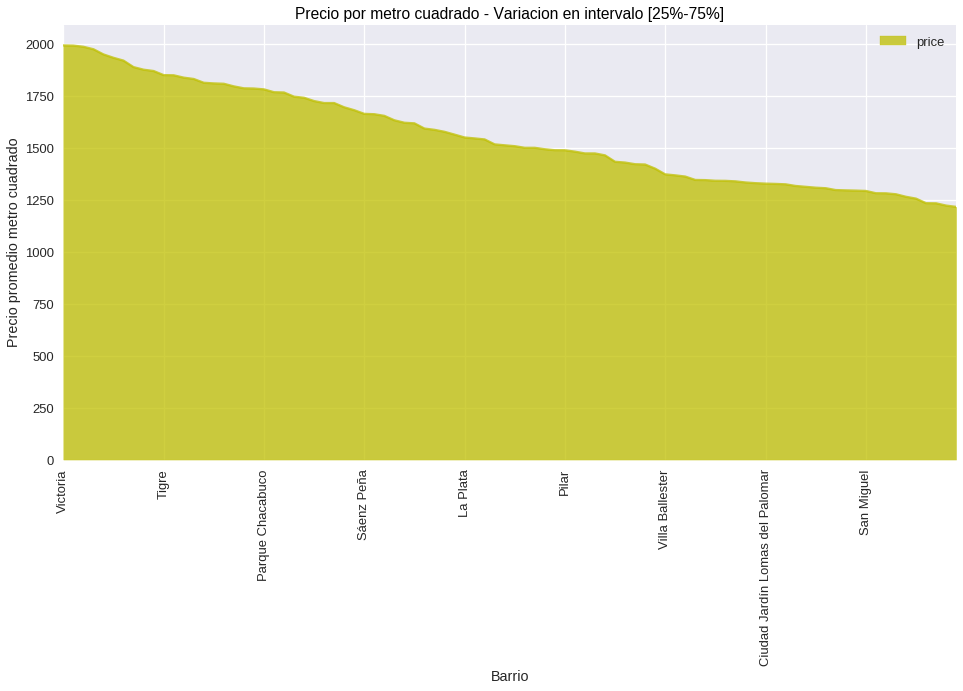
\includegraphics[width=7in, height=3.5in]{images/m2MiddleValues}
		  		\end{center}
		  		\tab  En el gráfico se aprecia lo mencionado previamente. El descenso es suave y, luego de cien barrios, 
		  		el precio cae sólo en (aproximadamente) $750USD$. \\
			\subsection{Análisis Global}
				Finalmente haremos un análisis global, nuevamente con un gráfico de area, dividiendo por sectores a todos los
				barrios. Desplazandonos desde el rojo (más caro) hasta el verde (más barato) mostramos cómo es la variación para
				cada rango de precios, analizando así en que sector es más suave la variación.
				\begin{center}
    					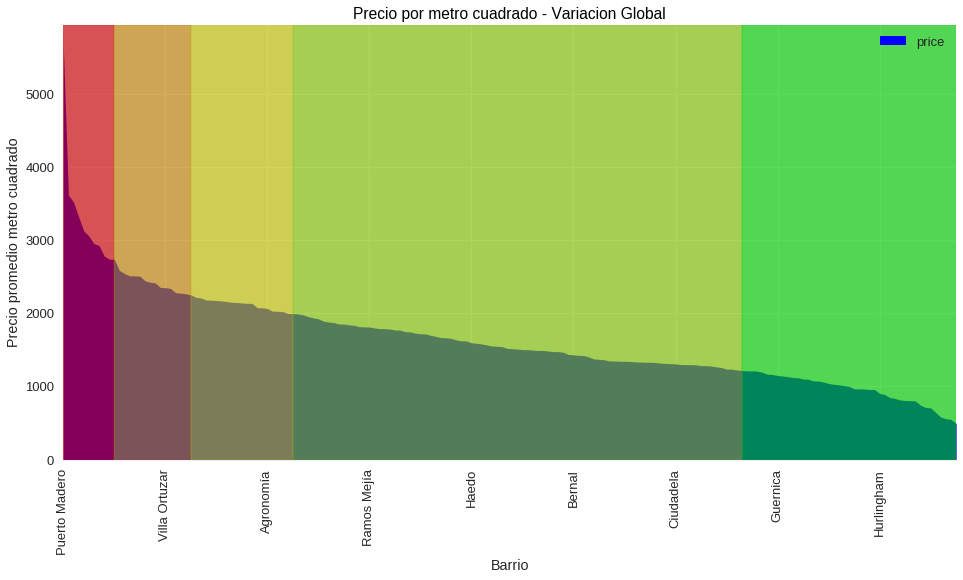
\includegraphics[width=7in, height=3.5in]{images/m2GlobalVariation}
		  		\end{center}
				\tab Más adelante complementaremos este análisis con \emph{Heat-Maps} de CABA y GBA, con los que podremos
				tener una mejor visualización tanto de la variación de los precios como de la ubicación de los barrios 
				con mayores y menores precios. \\		

\end{document}